\documentclass[11pt]{report}
\usepackage[utf8]{inputenc}
\usepackage[margin=2.0cm]{geometry}
\usepackage{tikz}
\usepackage{fancyhdr}
\usepackage{xcolor}
\usepackage{minted}
\usepackage{graphicx}
\usepackage[parfill]{parskip}
\usepackage{lscape}
\usepackage{multirow}

\usetikzlibrary{automata, positioning, arrows, fit}

\title{Digital Engineering\\Project Task 1}
\author{Y3890959\\Y3878784}
\date{28th February 2023}

\pagestyle{fancy}
\fancyhead{}
\setlength{\headheight}{14pt}
\fancyhead[L]{Project Task 1}
\fancyhead[R]{Y3890959, Y3878784}
\fancyfoot{}
\fancyfoot[L]{Digital Engineering}
\fancyfoot[R]{\thepage}

\makeatletter
\let\ps@plain\ps@fancy 
\makeatother

\setminted {
    fontsize=\footnotesize,
    frame=single,
}

\begin{document}

\maketitle

\chapter*{Task 1: Clock management through enable signals}

\section*{1 - FSM Description}

\begin{figure}[ht] % ’ht’ tells LaTeX to place the figure ’here’ or at the top of the page
    \centering % centers the figure
    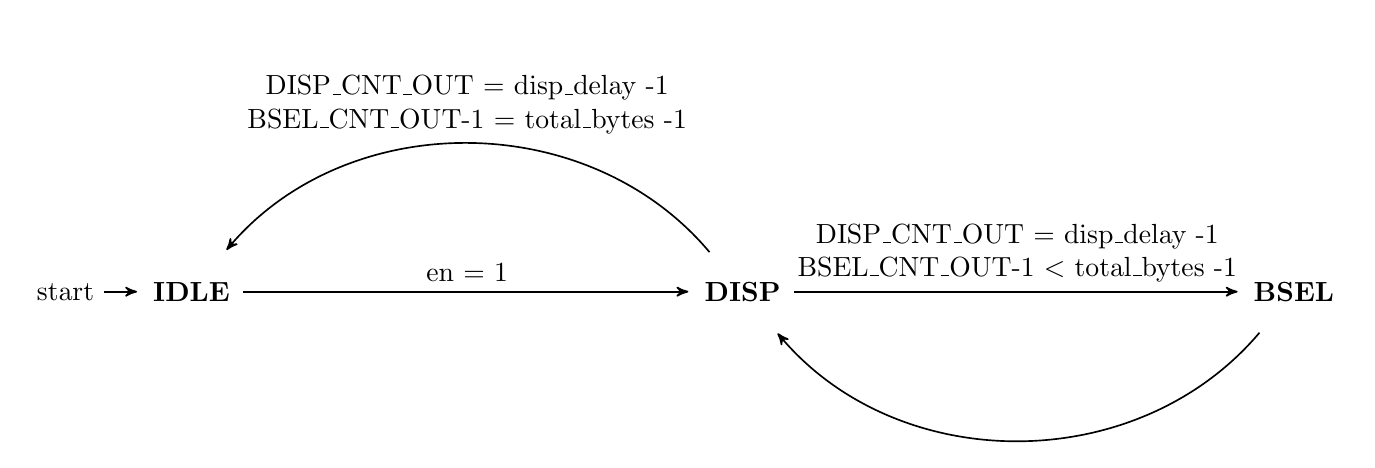
\begin{tikzpicture}[->,>=stealth',shorten >=1pt,auto,node distance=7cm,semithick]
        \tikzstyle{every state}=[draw=none,text=black]

        \node[initial,state] (A)              {\textbf{IDLE}};;
        \node[state]         (B) [right of=A] {\textbf{DISP}};
        \node[state]         (C) [right of=B] {\textbf{BSEL}};

        \path (A) edge                         node {en = 1} (B)
              (B) edge                         node[align=center] {DISP\_CNT\_OUT $=$ disp\_delay -1\\BSEL\_CNT\_OUT-1 $<$ total\_bytes -1} (C)
                  edge [above, bend right=50]  node[align=center] {DISP\_CNT\_OUT $=$ disp\_delay -1\\BSEL\_CNT\_OUT-1 $=$ total\_bytes -1} (A)
              (C) edge [below, bend left=50]   (B);
    \end{tikzpicture}
    \caption{FSM state graph}
    \label{fig:my_label}
\end{figure}
    
The FSM starts in the IDLE state, when the user presses the enable `en' pushbutton,
the state goes to DISP. As soon as the DISP state is reached, and the
DISP\_CNT for the LED delay and BSEL\_CNT byte index counter are reset
to 0, `EN\_SOURCE' goes high computing the next value in the sequence. Once the display
delay has reached its max value and there are still more bytes to display, the BSEL state
is selected, otherwise, once the delay is complete and all bytes have been displayed, the
logic goes back to the IDLE state. In the BSEL state, the BSEL counter is incremented.

\newpage
% Please add the following required packages to your document preamble:

\begin{landscape}
    \begin{table}[]
    \centering
    \resizebox{\columnwidth}{!}{%
    \begin{tabular}{|l|l|l|l|l|l|l|}
    \hline
    \textbf{STATE} &
      \textit{\textbf{EN\_SOURCE}} &
      \textit{\textbf{DISP\_CNT\_EN}} &
      \textit{\textbf{DISP\_CNT\_RST}} &
      \textit{\textbf{BSEL\_CNT\_EN}} &
      \textit{\textbf{BSEL\_CNT\_RST}} &
      \textit{\textbf{LED\_DISPLAY}} \\ \hline
    IDLE & 0                            & 0 & 1 & 0 & 1 & 00000000                                                                                    \\ \hline
    \multirow{4}{*}{DISP} &
      \multirow{2}{*}{\begin{tabular}[c]{@{}l@{}}1 when DISP\_CNT\_OUT \\ and DISP\_CNT\_OUT = 0\end{tabular}} &
      \multirow{4}{*}{1} &
      \multirow{4}{*}{0} &
      \multirow{4}{*}{0} &
      \multirow{4}{*}{0} &
      \begin{tabular}[c]{@{}l@{}}SOURCE\_DATA{[}7:0{]}\\ when DISPL\_CNT\_OUT is 0\end{tabular} \\ \cline{7-7} 
         &                              &   &   &   &   & \begin{tabular}[c]{@{}l@{}}SOURCE\_DATA{[}15:8{]}\\ when DISPL\_CNT\_OUT is 1\end{tabular}  \\ \cline{2-2} \cline{7-7} 
         & \multirow{2}{*}{0 otherwise} &   &   &   &   & \begin{tabular}[c]{@{}l@{}}SOURCE\_DATA{[}23:16{]}\\ when DISPL\_CNT\_OUT is 2\end{tabular} \\ \cline{7-7} 
         &                              &   &   &   &   & \begin{tabular}[c]{@{}l@{}}SOURCE\_DATA{[}31:24{]}\\ when DISPL\_CNT\_OUT is 3\end{tabular} \\ \hline
    BSEL & 0                            & 0 & 1 & 1 & 0 & 00000000                                                                                    \\ \hline
    \end{tabular}%
    }
    \caption{FSM table of outputs}
\end{table}
\end{landscape}
\newpage



\end{document}
